\documentclass[10pt, aspectratio=169]{beamer}

\usetheme{ugoe}
% Keeping graphics nice and tidy in a subfolder
\graphicspath{{./images/}{./}{/home/chris/Documents/PhD/Presentations/common_images/}}


% In general, you should encode all files using UTF-8
\usepackage[utf8]{inputenc}
\usepackage[T1]{fontenc}

% Set the math mode font to sans-serif
\let\mathrm\mathsf

% Use this for better font scaling (esp. if you want to use \tiny)
\usepackage{lmodern}
\usepackage{bm}
\usepackage{exscale}
\usepackage[normalem]{ulem}

\usepackage{multirow}
\usepackage{booktabs}
%\usepackage{ctable}
\usepackage{ragged2e}

\usepackage[yearmonthsep={-}, monthdaysep={-}, style=default]{datetime2}

\usepackage{xspace}
\usepackage{commath}
\usepackage{amsmath,amssymb}

\usepackage{siunitx}
\sisetup{separate-uncertainty = true, multi-part-units=single, list-final-separator = {,\;}, list-separator = {,\;}, list-pair-separator = {,~\mathrm{and}~}, exponent-product=\cdot}
\DeclareSIUnit{\lightspeed}{c}
\DeclareSIUnit{\electronvolt}{{e}\kern-0.08em{V}}
\DeclareSIUnit{\evmass}{\electronvolt\per\lightspeed\squared}
\DeclareSIUnit{\evmom}{\electronvolt\per\lightspeed}

\usepackage{tabularx}
\newcolumntype{C}[1]{%
    >{\setlength{\baselineskip}{0.8\baselineskip}
    \centering\arraybackslash}m{#1}
    }
\newcolumntype{L}[1]{%
    >{\setlength{\baselineskip}{0.8\baselineskip}
    \raggedright\arraybackslash}m{#1}
    }
\newcolumntype{R}[1]{%
    >{\setlength{\baselineskip}{0.8\baselineskip}
    \raggedleft\arraybackslash}m{#1}
    }
\newcolumntype{Y}{
    >{\setlength{\baselineskip}{0.8\baselineskip}
    \centering\arraybackslash}X
    }

\usepackage[compat=1.1.0]{tikz-feynman}

\usepackage{enumitem}
\setlist[itemize]{font=\color{ugoelogodark}}
\setlist[itemize,1]{label=$\bullet$}
\setlist[itemize,2]{label=--}
\setlist[enumerate]{font=\color{ugoelogodark}}
\setlist[enumerate,1]{label=\arabic*.}

%\usetikzlibrary{calc}

\newcommand\Overline[2][1pt]{%
  \begin{tikzpicture}[baseline=(a.base)]
    \node[inner xsep=0pt,inner ysep=1.5pt] (a) {$#2$};
    \draw[line width= #1] (a.north west) -- (a.north east);
  \end{tikzpicture}
}
\newcommand\textoverline[2][0.05em]{%
  \kern-0.05em
  \begin{tikzpicture}[baseline=(a.base)]
    \node[inner xsep=0pt,inner ysep=1.5pt] (a) {#2};
    \draw[line width= #1] ([yshift=0ex]a.north west) -- ([yshift=0ex]a.north east);
  \end{tikzpicture}
  \kern-0.37em
}
\newcommand{\textboldoverline}[2][0.07em]{
  \kern-0.35em
  \begin{tikzpicture}[baseline=(a.base)]
    \node[outer xsep=0pt, inner xsep=0pt,inner ysep=1.5pt] (a) {#2};
    \draw[line width= #1] (a.north west) -- (a.north east);
  \end{tikzpicture}
  \kern-0.35em
}

%\newcommand*{\textboldoverline}[1]{$\bm\bar{\mbox{#1}}$}
%\newcommand*{\textoverline}[1]{$\overline{\mathrm{#1}}$}
\newcommand*{\highl}[1]{\textbf{\color{ugoelogodark}#1}}

\newcommand{\dzero}      {D\O\xspace}
\newcommand{\cdf}        {CDF\xspace}
\newcommand{\uubar}      {\mbox{u\textoverline{u}}\xspace}
\newcommand{\ddbar}      {\mbox{d\textoverline{d\kern0.05em}\kern-0.05em}\xspace}
\newcommand{\ccbar}      {\mbox{c\kern-0.02em\textoverline{\kern0.02em{}c\kern0.02em}\kern-0.02em}\xspace}
\newcommand{\ssbar}      {\mbox{s\kern-0.02em\textoverline{\kern0.02em{}s\kern0.02em}\kern-0.02em}\xspace}
\newcommand{\ttbar}      {\mbox{t\kern-0.02em\textoverline{\kern0.05em{}t}}\xspace}
\newcommand{\bbbar}      {\mbox{b\kern-0.05em\textoverline{\kern0.05em{}b}}\xspace}
\newcommand{\ccbarbold}  {\mbox{\textbf{c\kern-0.02em\textboldoverline{\kern0.02em{}c\kern0.02em}\kern-0.02em}}\xspace}
\newcommand{\ttbarbold}  {\mbox{\textbf{t\kern-0.05em\textboldoverline{\kern0.05em{}t}}}\xspace}
\newcommand{\bbbarbold}  {\mbox{\textbf{b\kern-0.05em\textboldoverline{\kern0.05em{}b}}}\xspace}

\newcommand{\wjets}      {\mbox{W\,+\,4\;jets}\xspace}
\newcommand{\pttbar}     {\mbox{p\textsubscript{\ttbar}}\xspace}
\newcommand{\pwjets}     {\mbox{p\textsubscript{W\,+\,4\;jets}}\xspace}
\newcommand{\ljets}      {\mbox{$\ell$\,+\,jets}\xspace}
\newcommand{\ejets}      {\mbox{e\,+\,jets}\xspace}
\newcommand{\mujets}     {\mbox{$\mu$\,+\,jets}\xspace}
\newcommand{\ttjets}     {\mbox{\ttbar{}\,+\,jets}\xspace}
\newcommand{\ttljets}    {\mbox{\ttbar{}\,+\,light jets}\xspace}
\newcommand{\ttlight}    {\mbox{\ttbar{}\,+\,light}\xspace}
\newcommand{\ttc}        {\mbox{\ttbar{}\,+\,c}\xspace}
\newcommand{\ttb}        {\mbox{\ttbar{}\,+\,b}\xspace}
\newcommand{\wt}         {\mbox{Wt}\xspace}

\newcommand{\ttx}        {\mbox{\ttbar{}X}\xspace}
\newcommand{\ttv}        {\mbox{\ttbar{}V}\xspace}
\newcommand{\thiggs}     {\mbox{tH}\xspace}
\newcommand{\tth}        {\mbox{\ttbar{}H}\xspace}
\newcommand{\hbb}        {\mbox{H\,$\rightarrow$\,\bbbar}\xspace}
\newcommand{\thbb}       {\mbox{\thiggs{}(\hbb)}\xspace}
\newcommand{\tthbb}      {\mbox{\tth{}(\hbb)}\xspace}
\newcommand{\tthgam}     {\mbox{\tth{}(H\,$\rightarrow$\,$\gamma\gamma$)}\xspace}
\newcommand{\ttbb}       {\mbox{\ttbar{}\,+\,\bbbar}\xspace}

\newcommand{\thiggsbold} {\mbox{\textbf{tH}}\xspace}
\newcommand{\tthbold}    {\mbox{\ttbarbold{}\textbf{H}}\xspace}
\newcommand{\hbbbold}    {\mbox{\textbf{H}\,$\boldsymbol{\rightarrow}$\,\bbbarbold}\xspace}
\newcommand{\thbbbold}   {\mbox{\thiggsbold{}\textbf{(}\hbbbold{}\textbf{)}}\xspace}
\newcommand{\tthbbbold}  {\mbox{\tthbold{}\textbf{(}\hbbbold{}\textbf{)}}\xspace}

\newcommand{\thiggstitle}{\mbox{tH}\xspace}
\newcommand{\tthtitle}   {\mbox{t\kern-0.02em$\overline{\kern0.05em{}\mathrm{t}}$H}\xspace}
\newcommand{\hbbtitle}   {\mbox{H\,$\rightarrow$\,b\kern-0.05em$\overline{\kern0.05em{}\mathrm{b}}$}\xspace}
\newcommand{\tthbbtitle} {\mbox{\tthtitle{}(\hbbtitle)}\xspace}

\newcommand{\pt}         {\mbox{$p_{\kern0.1em\mathrm{T}}$}\xspace}
\newcommand{\mathpt}     {p_{\kern0.1em\mathrm{T}}}


\AtEndPreamble{\hypersetup{
pdftitle={},
pdfsubject={},
pdfauthor={},
pdfkeywords={}
}}

\title{\Large\color{ugoelogodark} BSc Intro 2022 ROOT Intro}
\shorttitle{ROOT Intro}
\author[]{Wael Alkakhi, Ishan Pokharel, Chris Scheulen, Sreelakshmi Sindhi}
\institute[Univ. of G\"ottingen]{II.~Physikalisches Institut, Georg-August-Universit\"at G\"ottingen}
\date{2022-03-09}

\def\insertlogos{
%   \centering
%   
\includegraphics[height=1.1cm]{logos/BMBF-Gef-Logo-gefoerdert.jpg}%
%   \hspace{0.5cm}%
%   \includegraphics[height=1.1cm]{logos/FSP_ATLAS.png}%
%   \end{minipage}
}

\begin{document}

\begin{frame}
  \titlepage
\end{frame}

\begin{frame}{Today's Agenda}

  \begin{itemize}
    \item
    \textbf{Intro}
    \begin{itemize}
      \item[--] Setting up
      \item[--] Interactive ROOT sessions
      \item[--] ROOT via Terminal
    \end{itemize}
    \item
    \textbf{Tutorial}
    \begin{itemize}
      \item[--] Opening TFiles
      \item[--] Creating TChains
      \item[--] Accessing Variables from TBranches
      \item[--] Setting up Event Loops
      \item[--] Filling Histograms (TH1/TH2)
      \item[--] Writing Histograms to TFile
      \item[--] General Notes
    \end{itemize}
  \end{itemize}
\end{frame}

\begin{frame}{First Things First: Setting Up}
  \normalsize
  \begin{enumerate}
    \item
      SSH into lxplus: \\ \textbf{\texttt{\$ ssh -XY <MY\_USERNAME>@lxplus.cern.ch}}
    \begin{itemize}
      \item[--] Flags for allowing graphical stuff (X11-Forwarding)
      \item[--] Hope you didn't forget your password here\ldots
    \end{itemize}
    \item
      setup ATLAS environment: \textbf{\texttt{setupATLAS}}
    \item
      Load up ROOT: \\ \textbf{\texttt{\$ lsetup "root <version>"}}
    \begin{itemize}
      \item[--] For looking up available versions: Use \textbf{\texttt{\$ showVersions root}}
      \item[--] Here: We will use version \textbf{6.20.06-x86\_64-centos7-gcc8-opt}
      \item[--] Later: Ask your \sout{doctor} supervisor, which version is right for you
    \end{itemize}
  \end{enumerate}
  \large Congrats! Now you are ready to ROOT!
\end{frame}

\begin{frame}{Interactive Mode}
  \begin{itemize}
    \item
      Simplest way to run ROOT: Interactive mode
    \begin{itemize}
      \item[--] Similar to python console
    \end{itemize}
    \item[$\rightarrow$]
      Just type \textbf{\texttt{root}} for this
    \begin{itemize}
      \item[--] Not ideal for running a full analysis (You'd have to remember every command in the right order\ldots)
      \item[--] Great for learning/debugging though
      \item[--] If you want to save many histograms: Batch-mode is your friend (Flag \textbf{\texttt{-b}} for this)
      \item[--] Annoyed by all the info? Flag \textbf{\texttt{-l}} to start quietly.
    \end{itemize}
    \item
      Now you can try out ROOT (and C++) commands
    \item
      Stuck in interactive mode with no way out?! \textbf{\texttt{.q}} to quit or \textbf{\texttt{.help}} to get help!
  \end{itemize}
\end{frame}

\begin{frame}{Stuff to Try Out}
  \begin{itemize}
    \item
      Define variables and use them (in C++ syntax)
    \begin{itemize}
      \item[--] \textbf{\texttt{double pi = 3.14}}
      \item[--] \textbf{\texttt{int r = 10}}
      \item[--] \textbf{\texttt{std::string "Welcome to ROOT!"}} ($\leftarrow$ Note how some C++ stuff works as well!)
      \item[--] \textbf{\texttt{2 * pi * r}}
    \end{itemize}
    \item
      Write a function (Multi-line expressions in brackets work!)
    \begin{itemize}
      \item[--] \textbf{\texttt{std::cout << "Hello, World!" << std::endl}}
      \item[--] \textbf{\texttt{[0] int doubling(int a) \{}} \\
                \textbf{\texttt{[1] return 2 * a;}} \\
                \textbf{\texttt{[2] \}}}
      \item[--] You need to include semicolons in multi-line functions (like in normal C++)!
    \end{itemize}
  \end{itemize}
  
\end{frame}

\begin{frame}{TBrowser}
  \begin{columns}
    \begin{column}{0.49\textwidth}
  \begin{itemize}
    \item
      Nice way of browsing through ROOT files
    \item
      Can show histograms, TTrees, etc.
    \item
      Also possible to modify attributes (e.g.~Histogram display options)
    \item
      A note on TTrees, TBranches and TLeaves:
    \begin{itemize}
      \item[--]
        Event data organized in TTrees
      \item[--]
        TTrees hold TBranches
      \item[--]
        Branches have TLeaves with the event variables (one variable per leaf, one or more leaves per branch)
    \end{itemize}
  \end{itemize}
    \end{column}
    \hfill
    \begin{column}{0.49\textwidth}
      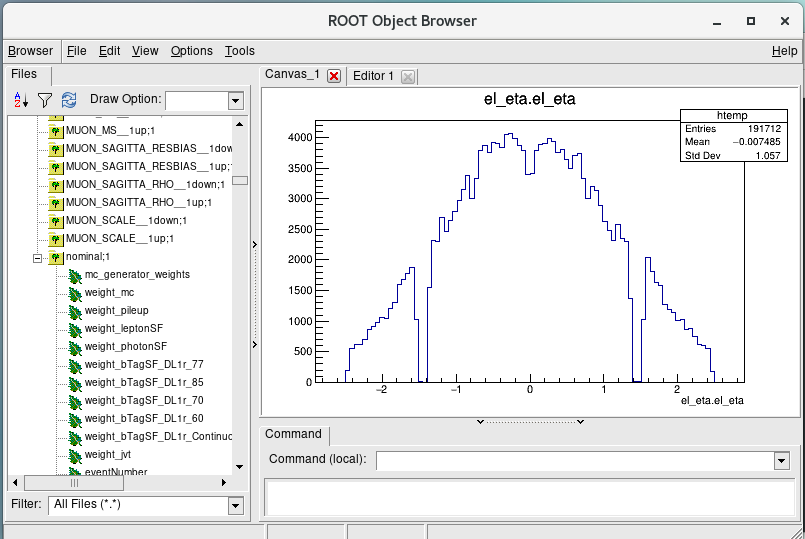
\includegraphics[width=\textwidth]{tbrow_example.png}
    \end{column}
  \end{columns}
\end{frame}

\begin{frame}{Looking at TFiles without TBrowser}
  \begin{itemize}
    \item
      You can load TFiles when starting ROOT: \\ \textbf{\texttt{\$ root <filepath>}}
    \begin{itemize}
      \item[$\rightarrow$] TFile gets handle (normally: \textbf{\texttt{\_file0}})
      \item[--] Alternative while in ROOT (used later today): \\ \textbf{\texttt{[0] TFile* file = new TFile("<filepath>", "READ")}} \\ \textbf{\texttt{[1] TTree* tree = (TTree*)file->Get("<treename>")}}
      
    \end{itemize}
    \item
      Now you can look at the tree contents:
    \begin{itemize}
      \item[--] \textbf{\texttt{[0] nominal->Print()}} prints tree contents of nominal
      \item[--] \textbf{\texttt{[1] nominal->Show(10)}} prints out all variables of the 10\textsuperscript{th} entries in nominal
      \item[--] \textbf{\texttt{[2] nominal->Scan("jet\_pt:jet\_eta")}} prints out values for jet\_pt and jet\_eta of entries
       \item[--] \textbf{\texttt{[3] nominal->Scan("jet\_pt:jet\_eta", "", "colsize=XX")}} prints out values for jet\_pt and jet\_eta of entries and specifies range of characters to print
      \item[--] \textbf{\texttt{[4] nominal->MakeClass("Myclass")}} generates a C++ class to reproduce the nominal TTree \\ (helpful for figuring out variable types)
    \end{itemize}
  \end{itemize}
\end{frame}




\begin{frame}

  \begin{center}
  \ugoeAddLogo
  \Large\bfseries Beginning of Tutorial: \\
  \large Creating an EventLoop for $t\bar{t}\gamma$ events with selection cuts!
  \end{center}
\end{frame}

\begin{frame}{Tips}
	\begin{enumerate}
		\item
		Memory Management in ROOT
		\begin{itemize}
			\item[--] Has its own memory management system that is different than a specific programming language's garbage collector.
			\item[--] If a file is open (TFile), then all objects (TObjects) are 'owned' by this file. Important to free up the object to the global register to be used later (\textbf{\texttt{SetDirectory(0)}})
			\item[--] Always open a file, access the object and IMMEDIATELY close the file.
		\end{itemize}
		\item
		\texttt{TBrowser} over ssh connection is very slow to respond
		\begin{itemize}
			\item[--] Familiarise and use \texttt{tree->Print(), tree->Scan()} for quick review.
			\item[--] Get Event related information from \texttt{tree->MakeClass("myClass")}.
			\item[--] If coding in C++, make sure the exact same object type is being used.
		\end{itemize}
		\item
		Environment setup
		\begin{itemize}
			\item[--] Include \texttt{setupATLAS} and other ATLAS-specific setups (\texttt{lsetup}) in a bash script. Create an alias to set it up in your \texttt{\textbackslash.bashrc} 
			\item[--] Bash \texttt{alias} is your friend!
		\end{itemize}
	\end{enumerate}
\end{frame}


\end{document}
